% Created 2023-11-10 Fri 22:59
% Intended LaTeX compiler: pdflatex
\documentclass[11pt]{article}
\usepackage[utf8]{inputenc}
\usepackage[T1]{fontenc}
\usepackage{graphicx}
\usepackage{longtable}
\usepackage{wrapfig}
\usepackage{rotating}
\usepackage[normalem]{ulem}
\usepackage{amsmath}
\usepackage{amssymb}
\usepackage{capt-of}
\usepackage{hyperref}
\author{Agustín Alejandro Mota Hinojosa}
\date{\today}
\title{PL/SQL 4-4: Iterative Control: WHILE and FOR Loops}
\hypersetup{
 pdfauthor={Agustín Alejandro Mota Hinojosa},
 pdftitle={PL/SQL 4-4: Iterative Control: WHILE and FOR Loops},
 pdfkeywords={},
 pdfsubject={},
 pdfcreator={Emacs 29.1 (Org mode 9.7)}, 
 pdflang={English}}
\begin{document}

\maketitle
\tableofcontents

\section{Vocabulary}
\label{sec:org6332a30}

Repeats a sequence of statements until the controlling condition is no longer TRUE.

\textbf{WHILE Loop}

Repeats a sequence of statements until a set number of iterations have been completed.

\textbf{FOR Loop}
\section{Try it / Solve it}
\label{sec:org2c4fc92}

\begin{enumerate}
\item Write a PL/SQL block to display the country\textsubscript{id} and country\textsubscript{name} values from the COUNTRIES table for country\textsubscript{id} whose values range from 51 through 55. Use a WHILE loop. Increment a variable from 51 through 55. Test your variable to see when it reaches 55. EXIT the loop after you have displayed the 5 countries.
\begin{verbatim}
DECLARE
 v_country_id wf_countries.country_id%TYPE := 51;
 v_country_name wf_countries.country_name%TYPE;
BEGIN
 WHILE v_country_id <= 55 LOOP
  SELECT country_name INTO v_country_name
  FROM wf_countries
  WHERE country_id = v_country_id;
  DBMS_OUTPUT.PUT_LINE(v_country_id || ' ' || v_country_name);
  v_country_id := v_country_id + 1;
 END LOOP;
END;
\end{verbatim}

\item Write a PL/SQL block to display the country\textsubscript{id} and country\textsubscript{name} values from the COUNTRIES table for country\textsubscript{id} whose values range from 51 through 55 in the reverse order. Use a FOR loop.
\begin{verbatim}
DECLARE
 v_country_id wf_countries.country_id%TYPE;
 v_country_name wf_countries.country_name%TYPE;
BEGIN
 FOR v_country_id IN REVERSE 51..55 LOOP
  SELECT country_name INTO v_country_name
  FROM wf_countries
  WHERE country_id = v_country_id;
  DBMS_OUTPUT.PUT_LINE(v_country_id || ' ' || v_country_name);
 END LOOP;
END;
\end{verbatim}

\item Execute the following statements to build a new\textsubscript{emps} table.
\begin{verbatim}
DROP TABLE new_emps;
CREATE TABLE new_emps AS SELECT * FROM employees;
ALTER TABLE new_emps ADD stars VARCHAR2(50);
\end{verbatim}
\begin{enumerate}
\item Create a PL/SQL block that inserts an asterisk in the stars column for every whole \$1,000 of an employee’s salary. For example, if an employee has a salary of \$7,800, the string “*****” would be inserted, and, if an employee has a salary of \$3,100, the string “*” would be inserted.
\begin{verbatim}
DECLARE
 v_empno new_emps.employee_id%TYPE := 124;
 v_asterisk new_emps.stars%TYPE := NULL;
 v_sal_in_thousands new_emps.salary%TYPE;
BEGIN
 SELECT NVL(TRUNC(salary/1000), 0) INTO v_sal_in_thousands
 FROM new_emps WHERE employee_id = v_empno;
 FOR i IN 1..v_sal_in_thousands LOOP
 v_asterisk := v_asterisk || '*';
 END LOOP;
 UPDATE new_emps
 SET stars = v_asterisk
 WHERE employee_id = v_empno;
END;
\end{verbatim}
\item Test your code using employee\textsubscript{ids} 124 and 142, then confirm the results.

\begin{center}
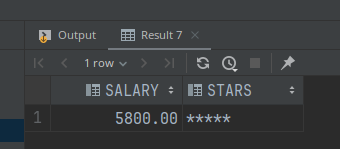
\includegraphics[width=.9\linewidth]{./resources/new_emps1.png}
\end{center}

\begin{center}
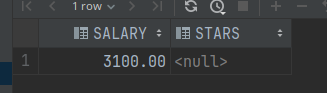
\includegraphics[width=.9\linewidth]{./resources/new_emps2.png}
\end{center}
\end{enumerate}
\end{enumerate}
\end{document}